\section{Máximo Exponente de Lyapunov}
\label{sec:MLE}

¿Que es lo que diferencia a un ciclo límite o una órbita cerrada de una órbita caótica? una órbita caótica (atractor caótico) es aperiódica, es decir que nunca se repite exactamente y la oscilación persiste para $t \to \infty$.
El movimiento sobre un atractor exhibe una dependencia sensible a las condiciones iniciales.
Esto significa que dos trayectorias que comienzan muy cercanas, rápidamente divergen una de otra, por lo que tendrán futuros muy diferentes.
La implicación práctica de esto es que la predicción a largo plazo se vuelve imposible en un sistema como este, en donde pequeñas incertezas son amplificadas rápidamente.
Hagamos estas ideas un poco más precisas.
Supongamos que te tenemos una trayectoria sobre el atractor y un punto $x(t)$ perteneciente a dicha trayectoria en un instante $t$, ahora consideremos un punto vecino $x(t) + \delta_0$, en donde $\delta_0$ es una pequeña separación inicial.
Ahora veamos como evoluciona esta separación $\delta(t)$.
Encontramos que
%
\begin{eqnarray}
\lVert \delta(t) \rVert \sim \lVert \delta_0 \rVert e^{\lambda t}
\end{eqnarray}
%
Por lo tanto, trayectorias vecinas se separan a un ritmo exponencial.
El número $\lambda$ es llamado exponente de Lyapunov.
Cuando este exponente es positivo, se dice que el sistema tiene un horizonte de tiempo $t_h$ más allá del cual la predicción falla por una tolerancia $a$, de modo que
%
\begin{eqnarray}
t_h \sim O ( \frac{1}{\lambda} \ln \frac{a}{\lVert \delta_0 \rVert})
\end{eqnarray}
%
Como este sistema presenta un horizonte de tiempo, puede decirse que es sensible a las condiciones iniciales, su exponente de Lyapunov es positivo y resulta ser caótico.

Los exponentes de Lyapunov son quantificadores que caracterizan como evoluciona la separación entre dos trayectorias \cite{Sprott2003}.
En general es bien conocido que el comportamiento caótico está principalmente caracterizado por los números de Lyapunov de la dinamica del sistema.

Venimos llamando al número $\lambda$ exponente de Lyapunov, sin embargo este es un uso poco riguroso de este término, por dos razones:
Primero, $\lambda$ depende de la trayectoria que estamos estudiando, deberíamos promediar sobre muchos puntos sobre la misma trayectoria para obtener su verdadero valor.
Segundo, realmente hay tantos exponentes de Lyapunov como dimensiones tenga el sistema.
Supongamos la evolución de una esfera infinitesimal de condiciones iniciales en el espacio de estados de tres dimensiones.
Durante esta evolución la esfera se se vuelve un elipsoide infinitesimal con tres ejes principales $\lambda_1$, $\lambda_2$ y $\lambda_3$, siendo estos tres los exponentes de Lyapunov del sistema.
El caos está definido por el máximo exponente de Lyapunov, a partir de ahora MLE, entonces basta que uno de los tres exponentes sea positivo para que el sistema sea caótico.
Si uno o mas números de Lyapunov es mayor que cero, entonces el sistema se comporta caóticamente, de otra forma el sistema es estable.

El Máximo Exponente de Lyapunov (MLE) caracteriza que tan rápido se apartan dos trayectorias.
Si esta velocidad es exponencial, se dice que el sistema es caótico, por lo que este exponente es conocido como un detector de  ``caoticidad", \cite{strotgartz1994,Kantz1994,Sprott2003}.
Más adelante, el MLE fue utilizado en diversas aplicaciones de muy distintas áreas.
Sólo por mencionar alguna, en \cite{Ma2013} el MLE es usado para medir una señal muy débil en un gas ideal utilizando criterios caóticos.
En \cite{Bruijna2011}, se estudia si es posible predecir un cambio en la probabilidad de caída para un modelo simple de caminante humano a partir del $MLE$.

Sabemos que el sistema en tiempo continuo es una idealización, por lo que se usa el exponente de Lyapunov para tiempo discreto:
%
\begin{eqnarray}
\label{eq:LtdiscB2}
	L = \lim\limits_{n \to \infty} \frac{1}{n} \sum_{i=1}^{n} \log_2 J_F(x,y,z)
\end{eqnarray}
%
en donde $L$ es un vector columna de tres dimensiones que contiene los tres exponentes de Lyapunov y $J_F(x,y,z)$ es la matriz jacobiana de la función $F$ para las variables $(x,y,z)$.
El logaritmo es en base dos para estimar la velocidad de apartamiento en bits.
Con estas dos consideraciones (tiempo discreto y base numérica binaria finita) la distancia entre dos trayectorias cambia en $2^{MLE}$ por cada iteración, en promedio.
Si el $MLE<0$ las trayectorias se aproximan, esto puede deberse a un punto fijo.
Si el $MLE=0$ las trayectorias mantienen su distancia, esto puede deberse a un ciclo límite.
Si el $MLE>0$ la distancia entre las trayectorias es creciente, lo que es un indicador de caos.

Calcular $L$ con la ecuación \ref{eq:LtdiscB2} tiene dos problemas:
Se necesitan infinitas iteraciones para hallar los exponentes de Lyapunov.
Trabajar con el jacobiano puede ser computacionalmente pesado, o éste puede no existir.
Afortunadamente existe un algoritmo no analítico por aproximaciones sucesivas que converge al máximo exponente de Lyapunov.
Las entradas y las salidas de un sistema deben ser accesibles para poder utilizarlo.
El procedimiento es el siguiente: el sistema debe ser iniciado desde dos puntos cercanos en el plano de fase, llamémoslos $(x_a,y_a)$ y $(x_b,y_b)$.
A medida que el sistema es iterado se mide la distancia euclideana entre las dos trayectorias ($d_n$ en la muestra $n_{th}$) (eq. \ref{eq:D0D1}), y la trayectoria $b$ es relocalizada en cada iteración (eq. \ref{eq:reubicacion}) obteniendo los puntos $(x_{br},y_{br})$ para realimentar el sistema.
Entonces, el MLE puede ser calculado como se muestra en la ecuación \ref{eq:Lyapunov}.
El proceso puede verse en la Fig. \ref{fig:relocalizacion}.

\begin{eqnarray}\label{eq:D0D1}
d_{0(i-1)}&=& \sqrt{(x_{a(i-1)}-x_{br(i-1)})^2+(y_{a(i-1)}-y_{br(i-1)})^2}\nonumber\\
d_{1(i)}&=& \sqrt{(x_{a(i)}-x_{b(i)})^2+(y_{a(i)}-y_{b(i)})^2}\\
\nonumber
\end{eqnarray}

\begin{eqnarray}\label{eq:Lyapunov}
MLE &=& \frac{1}{n} \sum_{i=2}^{n} \log_2{\frac{d_{1(i)}}{d_{0(i-1)}}}
\end{eqnarray}

\begin{eqnarray}\label{eq:reubicacion}
x_{br(i)}&=& x_{a(i)}+(x_{b(i)}-x_{a(i)})d_{o(i-1)}/d_{1(i)} \nonumber\\
y_{br(i)}&=& y_{a(i)}+(y_{b(i)}-y_{a(i)})d_{o(i-1)}/d_{1(i)}
\end{eqnarray}

\begin{figure}
	\centering
	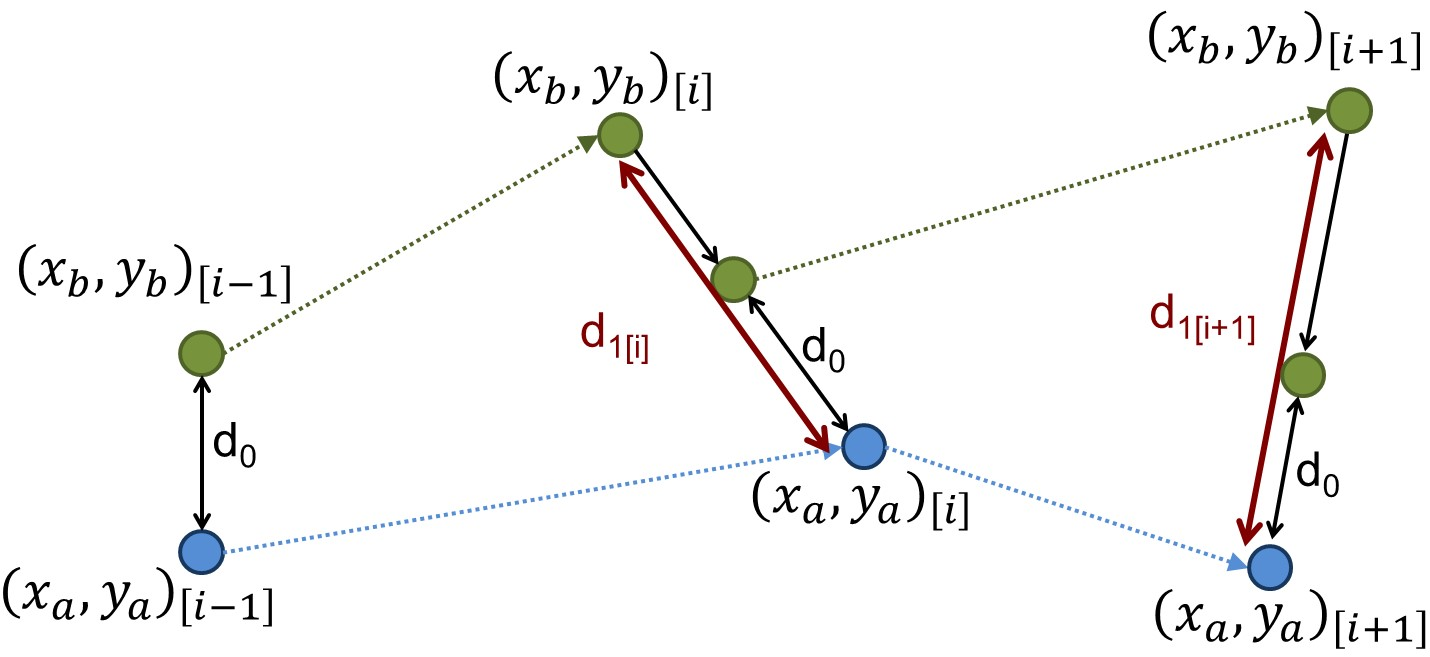
\includegraphics[width=1\columnwidth]{relocalizacion}\\
	\caption{Algoritmo para calcular el MLE.}\label{fig:relocalizacion}
\end{figure}

